%
% teil1.tex -- Beispiel-File für das Paper
%
% (c) 2020 Prof Dr Andreas Müller, Hochschule Rapperswil
%
%
% teil2.tex -- Beispiel-File für teil2 
%
% (c) 2020 Prof Dr Andreas Müller, Hochschule Rapperswil
%



\section{Kalman Filter}
\subsection{Geschichte}
Das Kalman Filter wurde 1960 von Rudolf Emil Kalman entdeckt und direkt von der NASA für die Appollo Mission benutzt. Der Filter kommt mit wenig Rechenleistung aus und war somit dafür geeignet die Rakete bei der Navigation zu unterstützen. Das Filter schätzt den Zustand eines Systems anhand von Messungen und kann den nächsten Zustand errechnen. Typische Anwendungen des Kalman-Filters sind die Glättung von verrauschten Daten und die Schätzung von Parametern und kommt heutzutage in jedem Satellit, Navigationssystem, Smartphones und Videospielen vor.

\subsection{Wahrscheinlichkeit}
Das Kalman Filter versucht nichts anderes, als ein geeigneter Wert zwischen zwei Normalverteilungen zu schätzen. Die eine Kurve zeigt die errechnete Vorhersage des Zustands, bzw. deren Normal- Gauss-Verteilung. Die andere Kurve zeigt die verrauschte Messung des nächsten Zustand, bzw. deren Normal-Verteilung. Wie man in am Beispiel dieser zwei Gauss-Verteilungen sehen kann, ist sowohl der geschätzte Zustand als auch der gemessene Zustand nicht am selben Punkt. 



\begin{figure}
 \begin{center}
 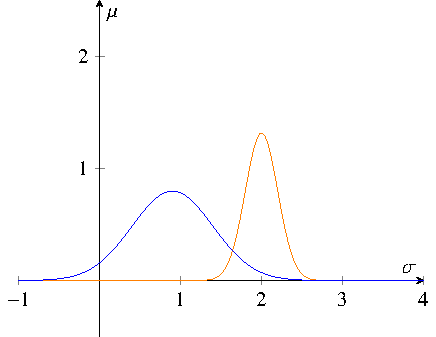
\includegraphics[width=5cm]{papers/erdbeben/Gausskurve2.pdf}
 \caption{System}
 \end{center}
\end{figure}



Um eine genauere Schätzung des Zustandes zu machen, wird nun ein Wert zwischen den beiden Verteilungen gesucht. An diesem Punkt wird nun eine Eigenschaft ausgenutzt. Durch das Multiplizieren zweier Normalverteilungen entsteht eine neue Normalverteilung. 

Wir haben eine Normalverteilung der Vorhersage:
\begin{equation}
{y_1}(x;{\mu_1},{\sigma_1})=\frac{1}{\sqrt{2\pi\sigma_1^2}}\quad e^{-\frac{(x-{\mu_1})^2}{2{\sigma_1}^2}}
\end{equation} 
und für die Messung:

\begin{equation}
{y_2}(x;{\mu_2},{\sigma_2})=\frac{1}{\sqrt{2\pi\sigma_2^2}}\quad e^{-\frac{(x-{\mu_2})^2}{2{\sigma_2}^2}}.
\end{equation} 

Diesen werden nun Multipliziert und durch deren Fläche geteilt um sie wieder zu Normieren:
\begin{equation}
{y_f}(x;{\mu_f},{\sigma_f})=\frac{ \frac{1}{\sqrt{2\pi\sigma_1^2}}e^{-\frac{(x-{\mu_1})^2}{2{\sigma_1}^2}} \cdot \frac{1}{\sqrt{2\pi\sigma_2^2}}e^{-\frac{(x-{\mu_2})^2}{2{\sigma_2}^2}}}{\int {y_1}*{y_2}\,}
\end{equation} 

Dadurch gleicht sich die neue Kurve den anderen an. Interessant daran ist, dass die fusionierte Kurve sich der genauere Normal-Verteilung anpasst. ist ${\sigma_2}$ klein und ${\sigma_1}$ gross, so wird sich die fusionierte Kurve näher an ${y_2}(x;{\mu_2},{\sigma_2})$ begeben. Sie ist also Gewichtet und die best mögliche Schätzung. 


\begin{figure}
 \begin{center}
 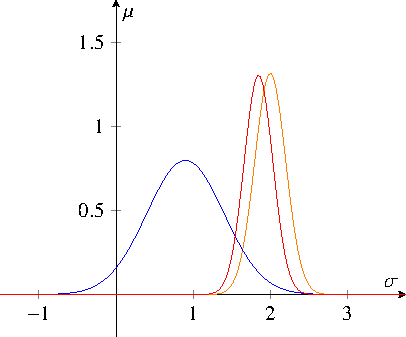
\includegraphics[width=5cm]{papers/erdbeben/Gausskurve3.pdf}
 \caption{System}
 \end{center}
\end{figure}

 
Was in 2 Dimensionen erklärt wurde, funktioniert auch in mehreren Dimensionen. Dieses Prinzip mach sich der Kalman Filter zu nutze, und wird von uns für die Erdbeben Berechnung genutzt. 

\subsection{Anwendungsgrenzen}
Nicht lineare Systeme %Noch nicht Fertig


\section{Aufbau}
Um ein Erdbeben kenntlich zumachen werden in der Regel Seismographen mit vielen Sensoren verwendet. 
Ein Seismograph besteht im Grunde aus einer federgelagerten Masse. Wirkt eine Bodenerregung auf das Gerät ein, bleibt die gekoppelte Masse in der regel stehen und das Gehäuse schwingt mit.Relativbewegung des Bodens kann damit als Längenänderung im Zeitverlauf gemessen werden. In modernen Seismographen wird die Bodenbewegung in alle Richtungen gemessen, sowohl Horizontal als auch Vertikal. 
Wir konstruieren uns eine einfachere Version eines Seismographen, welcher rein mechanisch funktioniert. Zudem kann er nur in eine Dimension Messwerte aufnehmen. Würde das System ausgebaut werden, um alle Horizontalbewegungen aufzunehmen, würde der Verwendung des Kalman-Filters zu kompliziert werden. Für zwei Dimensionen (x,y) würde der Pythagoras für das System benötigt werden. Da sich der Pythagoras bekanntlich nicht linear verhält, kann kein lineares Kalman-Filter implementiert werden. Da das Kalman-Filter besonders effektiv und einfach für lineare Abläufe geeignet ist, würde eine Zweidimensionale Betrachtung den Rahmen dieser Arbeit sprengen. Für ein nicht-lineares System werden Extended Kalman-Filter benötigt, bei denen die System-Matrix (A) durch die Jacobi-Matrix des System ersetzt wird.

\begin{figure}
 \begin{center}
 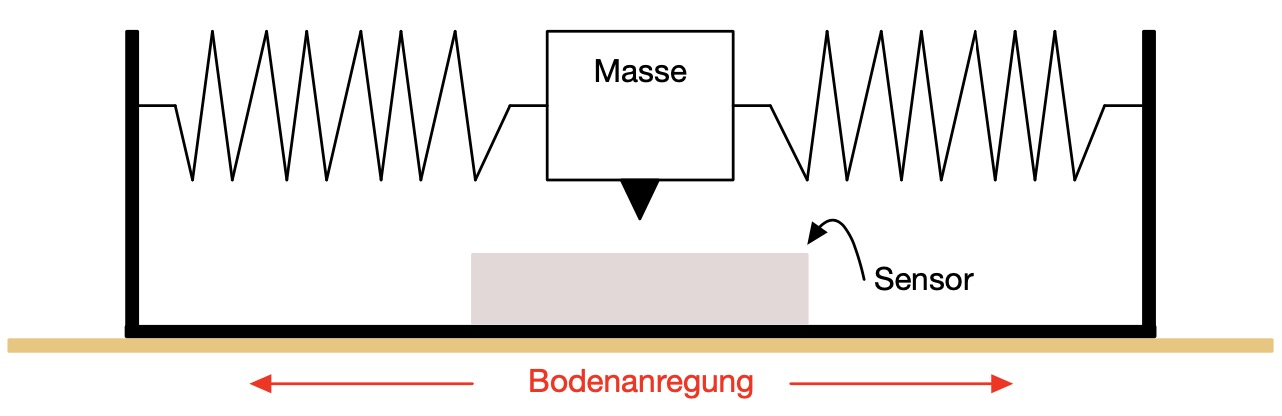
\includegraphics[width=5cm]{papers/erdbeben/Apperatur}
 \caption{System}
 \end{center}
\end{figure}


\subsection{Optionen}
Wollte man einen 2D Seismographen aufbauen, ohne den Pythagroas zu verwenden, kann dies mit der Annahme, das die Feder sehr lang sind erfolgen. Da sich bei langen Federn die Auslenkungen verkleiner...!!Noch nicht fertig!

\section{Systemgleichung}
Da das Kalman-Filter zum Schätzen des nächsten Zustand verwendet wird, wird eine Gleichung, welche das System beschreibt. Das Kalman-Filter benötigt eine Beschreibung der Systemdynamik. Im Fall unseres Seismographen, kann die Differentialgleichung zweiter Ordnung einer gedämpften Schwingung am harmonischen Oszillator verwendet werden. Diese lautet:
\begin{equation}
m\ddot x + 2k \dot x + Dx = f
\end{equation}
mit den Konstanten $m$ = Masse, $k$ = Dämpfungskonstante und $D$  = Federkonstante.
Um diese nun in die Systemmatrix umzuwandeln, wird aus der Differentialgleichung zweiter Ordnung durch eine Substitution eine DGL erster Ordnung:


\begin{equation}
{x_1}=x, \qquad
{x_2}=\dot x,  \qquad
{x_3}=\ddot x\qquad \mid \quad \text {Substitution}
\end{equation}


\begin{equation}
m{x_3}+ 2k{x_2} + D{x_1} = f\qquad \mid \quad \text {DGL 1. Ordnung}
\end{equation} 

\begin{equation}
{x_3}=-\frac{D}{m} {x_1} -\frac{2k}{m} {x_2} + \frac{f} {m}  \qquad \mid \quad \text {nach}  \quad{x_3} 
\end{equation} 
auch als Matrix-Vektor-Gleichung schreiben.
Hierbei beschreibt die Matrix $A$ die gesamte Systemdynamik in der Form, wie sie ein Kalman-Filter benötigt.

Um die lineare Differentialgleichung in das Kalman-Filter zu implementieren, muss dieses als Vektor-Gleichung umgewandelt werden. Dafür wird die Gleichung in die Zustände aufgeteilt. Die für uns relevanten Zustände sind die Position der Masse, die Geschwindigkeit der Masse und äussere Beschleunigung des ganzen System. Dabei muss unterschieden werden. um welche Beschleunigung es sich handelt. Das System beinhaltet sowohl eine Beschleunigung der Masse bzw. Feder (innere Beschleunigung), als auch eine Beschleunigung der ganzen Apparatur (äussere Beschleunigung). In unserem Fall wird die äusseren Beschleunigung gesucht, da diese der Erdbeben Anregung gleich kommt. 


\begin{equation}
\frac{d}{dt} \left(\begin{array}{c} {x_1} \\ {x_2}  \end{array}\right) = \left(
 \begin{array}{ccc} 	
0 & 1& 0 \\ 
- \frac{D}{m} &-\frac{2k}{m} & \frac{1} {m}\\
\end{array}\right)  \left(\begin{array}{c} {x_1} \\ {x_2} \\ {x_3} \end{array}\right).
\end{equation}

Durch die Rücksubstituion ergibt sich:
\begin{equation}
\frac{d}{dt} \left(\begin{array}{c} x(t) \\ v(t) \end{array}\right) = \left(
 \begin{array}{ccc} 	
0 & 1& 0 \\ 
- \frac{D}{m} &-\frac{2k}{m} & \frac{1} {m}\\
\end{array}\right)  \left(\begin{array}{c} x(t)\\ v(t)\\ f(t) \end{array}\right).
\end{equation}


Da die Kraft unbekannt ist, wird die letzte Zeile später mit Nullen bestückt, denn genau diese Werte wollen wir. 

\section{Kalman Filter}
Um den Kalman Filter zu starten, müssen gewisse Bedingungen definiert werden. In diesem Abschnitt werden die einzelnen Parameter/Matrizen erläutert und Erklärt, wofür sie nützlich sind. 


\subsection{Anfangsbedingungen}
\subsubsection*{Anfangszustand $x$}
Das Filter benötigt eine Anfangsbedingung. In unserem Fall ist es die Ruhelage, die Masse bewegt sich nicht. Zudem erföhrt die Apparatur keine äussere Kraft.

\begin{equation}
{x_0 }= \left( \begin{array}{c} 0\\ 0\\ 0\end{array}\right)
\end{equation} 

\subsubsection*{Anfangsfehler / Kovarianzmatrix $P$}
Da auch der Anfangszustand fehlerhaft sein kann, wird für den Filter einen Anfangsfehler eingeführt. Auf der Diagonalen werden die Varianzen eingesetzt, in den restlichen Felder stehen die Kovarianzen.
In unserem Fall ist der Anfangszustand gut bekannt. Wir gehen davon aus, dass das System in Ruhe und in Abwesenheit eines Erdbeben startet, somit kann die Matrix mit Nullen bestückt werden. Somit ergibt sich für die Kovarianzmatrix

\begin{equation}
{P_0 }=
\left(
\begin{array}{ccc} 	
0 & 0 &0 \\ 
0 &0 & 0 \\ 
0 & 0 &0 \\
\end{array}
\right).
\end{equation}
Diese Matrix beschreibt die Unsicherheit des geschätzten Zustandes und wird sowohl für die Vorhersage als auch die Korrektur benötigt. Sie wird nach jeder Schätzung aktualisiert.. Für einen gut bekannten Zustandsvektor können kleine Werte eingesetzt werden, für ungenaue Anfangsbedingungen sollten grosse Werte (1 Million) verwendet werden. Grosse Werte ermöglichen dem Filter sich schnell einzupendeln. 


\subsubsection*{Dynamikmatrix $A$}
Die Dynamikmatrix bildet den Kern des Filters. Diese wurde weiter oben Bereits beschrieben. Dabei wollen wird die äussere Kraft des Systems ermitteln.
Da nichts über die äussere Kraft bekannt ist, müssen wir annehmen das deren Ableitung 0 ist.
Die System Vektor-Gleichung lautet daher:


\begin{equation}
A = \left(
 \begin{array}{ccc} 	
0 & 1& 0 \\
- \frac{D}{m} &-\frac{2k}{m} & \frac{1} {m}\\
0 & 0& 0\\ 
\end{array}\right)  
\end{equation} 

\subsubsection*{Prozessrauschkovarianzmatrix $Q$}
Die Prozessrauschmatrix teilt dem Filter mit, wie sich der Systemzustand verändert. Kalman-Filter berücksichtigen Unsicherheiten wie Messfehler und -rauschen. Bei unserem Modell könnte das beispielsweise ein Windstoss an die Masse sein. Für uns wäre dies:
\begin{equation}
Q = \left(
 \begin{array}{ccc} 	
{\sigma_x }^2& 0& 0 \\ 
0 & {\sigma_v }^2& 0\\ 
0 & 0& {\sigma_f }^2\\
\end{array}\right)  
\end{equation} 

Die Standabweichungen müssten Statistisch ermittelt werden, da der Fehler nicht vom Sensor kommt und somit nicht vom Hersteller gegeben ist. Das Bedeutet wiederum dass $Q$ die Unsicherheit des Prozesses beschreibt, und die Messung. 

\subsubsection*{Messmatrix $H$}
Die Messmatrix gibt an, welcher Parameter gemessen werden soll. In unserem Fall ist es nur die Position der Massen. 

\[ H = (1, 0, 0) \]


\subsubsection*{Messrauschkovarianz $R$}
Die Messrauschkovarianzmatrix beinhaltet, wie der Name es schon sagt, das Rauschen der Positionssensoren. In unserem Fall wird nur die Position der Masse gemessen. Da wir keine anderen Sensoren haben ist dies lediglich:
\begin{equation}
R= ({\sigma_x}^2).
\end{equation} 
Diese Messrauchen wird meistens vom Sensorhersteller angegeben. Für unsere Theoretische Apparatur wird hier ein kleiner Fehler eingesetzt.

\subsection{Fiter Algorithmus}
Nachdem alle Parameter aufgestellt sind, wird der Filter initialisiert und wird den Zustand der Feder vorherzusagen, die Messung zu präzisieren und laufend zu aktualisieren. Das Filter berechnet aufgrund der aktuellen Schätzung eine Vorhersage. Diese wird, sobald verfügbar, mit der Messung verglichen. Aus dieser Differenz und den Unsicherheiten des Prozesses ($Q$) und der Messung ($R$) wird der wahrscheinlichste, neue Zustand geschätzt.


\subsubsection*{Vorhersage}
Im Filterschritt Vorhersage wird der nächste Zustand anhand des Anfangszustand und der Systemmatrix berechnet. Dies funktioniert ganz Trivial mit dem Rechenschritt:
\begin{equation}
{x_{t+1}}=A\cdot{x_t}.
\end{equation} 


Die Kovarianz $P_{pred}$ wird ebenfalls neu berechnet, da die Unsicherheit im Vorhersage grösser wird als im Aktuellen. Da wir ein mehrdimensionales System haben, kommt noch die Messunsicherheit $Q$ dazu, so dass die Unsicherheit des Anfangsfehlers $P$ immer grösser wird. Dies funktioniert durch multiplizieren der Systemmatrix, deren Ableitung und mit dem aktualisierten Anfangsfehler. Dazu wird noch die Messunsicherheit addiert, somit entsteht die Gleichung

\begin{equation}
{P_{pred}}=APA^T+Q.
\end{equation}

wird dieser Vorgang wiederholt, schaut der Filter wie genau die letzte Anpassung von $P$ zur Messung stimmt. Ist der Unterschied klein, wird die Kovarianz $P$ kleiner, ist der Unterschied gross, wird auch die Kovarianz grösser. Das Filter passt sich selber an und korrigiert sich bei grosser Abweichung.

\subsubsection*{Messen}
Der Sensor wurde noch nicht benutz, doch genau der liefert Werte für den Filter. Die aktuellen Messwerte $z$ werden die Innovation $w$ mit dem Zustandsvektor $x$ und der Messmatrix $H$ zusammengerechnet.
Hier bei wird lediglich die Messung mit dem Fehler behaftet, und die Messmatrix $H$ 
\begin{equation}
w=Z-(H\cdot x)
\end{equation}
Die Innovation ist der Teil der Messung, die nicht durch die Systemdynamik erklärt werden kann. 
Innovation = Messung - Vorhersage. Dies ist Intuitiv logisch, eine Innovation von 0 bedeutet, dass die Messung nichts Neues hervorbrachte.

Im nächsten Schritt wir analysiert, mit welcher Kovarianz weiter gerechnet wird. 

\subsubsection*{Korrigieren}
Udpdate
\section{Anfügen der Schwingung}

Ein Erdbeben breitet sich im Boden wellenartig aus und bringt Objekte, wie zum Beispiel ein Gebäude, in Schwingung.
Diese Schwingungen pflanzen sich im Gebäude mit gleicher Amplitude, Geschwindigkeit und Beschleunigung in horizontaler und vertikaler Bewegung fort.
Wir möchten herauszufinden, wie gross die Massenbeschleunigung infolge eines Erdbeben ist.
Mit Hilfe von fiktiven Sensoren, die eine Ortsveränderung des Gebäude messen, können wir mit Anwendung von Matrizen und dem Kalman-Filter die Beschleunigung berechnen.

\begin{equation}
\int_a^b x^2\, dx
=
\left[ \frac13 x^3 \right]_a^b
=
\frac{b^3-a^3}3.
\label{erdbeben:equation1}
\end{equation}

\section{Erreger-Schwingung}
Wir möchten mit einer gedämpften harmonischen Schwingung ein einfaches Erdbeben simulieren, die im Kalman Filter eingespeist wird.
Die Gleichung lautet

\begin{equation}
x(t)=Ae^{t/2}sin(t).
\end{equation}

Mit dieser Schwingung können wir ein einachsiger Seismograph simulieren, der eine Ortsverschiebung auf der x-Achse durchführt.
Die Dämpfung der Schwingung ist relevant, da das System beim Schwingungsvorgang durch die Federkonstante und der Reibung, Energie verliert.

Die Ergebnisse dieser Schwingung setzen wir in die Messmatrix ein und können den Kalman-Filter starten.




